\section{Numerical results}

\subsection{Implementation}

\paragraph{IPM solver.}
We have implemented the two condensed-space methods in our nonlinear IPM solver MadNLP~\cite{shin2021graph}.
This implementation utilizes the abstraction {\tt AbstractKKTSystem} to represent the various formulations of the KKT linear systems.
MadNLP is able to deport most of the IPM algorithm to the GPU, with the exception of basic IPM operations used for the coordination, such as the filter line-search algorithm.

\paragraph{Evaluation of the nonlinear models.}
We use the ExaModels.jl modeling tool~\cite{shin2023accelerating} to implement all the nonlinear programs utilized in our benchmark.
ExaModels.jl harnesses the implicit sparsity structure and provides custom derivative kernels for repetitive algebraic subexpressions of the constraints and objective functions to compute first and second-order derivatives on the GPU in parallel~\cite{bischof1991exploiting,enzyme2021}.
This approach caters to the SIMD architecture of the GPU by assigning each expression to multiple threads responsible for computing derivatives for different values.

\paragraph{Linear solvers.}
We factorize the KKT systems assembled within MadNLP using various sparse linear solvers, chosen based on the KKT formulation (K1, K2, K3) and the device (CPU, GPU) being utilized.
In particular, we utilize the following solvers:
\begin{itemize}
  \item {\tt HSL MA27}: Implements the \lblt factorization on the CPU.
    It solves the augmented KKT system~\eqref{eq:kkt:augmented}.
    This solver serves as the reference when running on the CPU.
  \item {\tt CHOLMOD}: Implements the Cholesky factorization on the CPU
    (using the AMD ordering \cite{amestoy-david-duff-2004} by default).
    It factorizes the condensed matrix $K_\gamma$ appearing in \eqref{eq:kkt:hykkt}.
    This solver is used to assess the performance of the Golub \& Greif strategy when running on the CPU.
  \item {\tt cuDSS}: Implement \llt, \ldlt and \lu decompositions on an NVIDIA GPU.
    We use the Cholesky factorization to factorize the condensed matrix $K_\gamma$ on GPU.
    This newly released solver is the contender in our benchmark.
  \item {\tt Krylov.jl}: Contains the CG method for both CPU and GPU architectures, as part of the Golub \& Greif strategy.
\end{itemize}

We use the Julia language \cite{bezanson-edelman-karpinski-shah-2017} for the comparison, where CHOLMOD \cite{chen-davis-hager-rajamanickam-2008} is included with Julia.
For the HSL linear solvers, we utilize libHSL \cite{fowkes-lister-montoison-orban-2024} with the Julia interface HSL.jl \cite{montoison-orban-hsl-2021}.
HSL MA27 and CHOLMOD are both compiled with OpenBLAS \cite{openblas}, a multithreaded version of BLAS and LAPACK.
The Julia package Krylov.jl~\cite{montoison2023krylov} contains a collection of Krylov methods with a polymorphic implementation that can be used on both CPU or GPU architectures.
% Should we provide the version of the linear solvers?

\subsection{Performance analysis on a large-scale instance}
We initially evaluate the performance of each KKT solver on a large-scale OPF instance, taken from
the PGLIB benchmark~\cite{babaeinejadsarookolaee2019power}: {\tt 78484epigrids}.
We have implemented the model in ExaModels.jl, to support
the evaluation of the GPU: our formulation has
a total of 85,568 variables, 82,679 equality constraints and 48,147
inequality constraints.jl.
It is acknowledged that this particular instance is challenging to solve
with IPM, as it requires a non-trivial amount of primal-dual regularization
to achieve convergence.
Our previous work has pointed out that the KKT solver is the current bottleneck
in the numerical implementation~\cite{shin2023accelerating}.

\subsubsection{Individual performance of the linear solvers}
Subsequently, we evaluate the individual performance of the cuDSS solver when factorizing the matrix $K_{\gamma}$ at the first IPM iteration (here with $\gamma = 10^7$).
We compare the analysis
time, the factorization time and the triangular solve time with CHOLMOD.
The results are displayed in Table~\ref{tab:linsol:time}. We benchmark the
three decompositions implemented in cuDSS (\llt, \ldlt, \lu), and look at
the accuracy obtained in the backsolve. We observe the analysis phase
is almost 10 times slower for cuDSS, compared to CHOLMOD.
That operation has to be computed only once, meaning that its cost is amortized if we run
many IPM iterations. The refactorization is about twice as fast in cuDSS,
with a time almost independent from the algorithm being used. The backsolve
is 3 times slower, as the triangular solve algorithm does not parallelize
well on a GPU. In terms of accuracy, the quality of the solution remains on
par with CHOLMOD, except for the \ldlt decomposition which lags behind by at least
2 orders of magnitude.


\begin{table}[!ht]
  \centering
  \resizebox{\textwidth}{!}{
  \begin{tabular}{|lrrrr|}
  \hline
  linear solver & analysis (s) & factorization (s) & backsolve (s) & accuracy \\
  \hline
    cholmod     & 0.798 &$6.34\times 10^{-1}$&$5.50\times 10^{-2}$&$3.60\times 10^{-13}$\\
    cudss-\llt  & 3.50  &$4.77\times 10^{-2}$&$2.08\times 10^{-2}$&$2.64\times 10^{-13}$\\
    cudss-\lu   & 3.48  &$4.97\times 10^{-2}$&$1.91\times 10^{-2}$&$2.58\times 10^{-13}$\\
    cudss-\ldlt & 3.49  &$5.80\times 10^{-2}$&$1.88\times 10^{-2}$&$5.44\times 10^{-11}$\\
  \hline
  \end{tabular}
  }
  \caption{Comparing the performance of cuDSS with CHOLMOD.
    The matrix $K_\gamma$ is symmetric positive definite, with
    a size $n = 85,568$. The matrix is extremely sparse, with only $1,057,200$ non-zero entries ($0.01$\%).
    \label{tab:linsol:time}
    (A30 GPU)
  }
\end{table}


\subsubsection{Tuning the Golub \& Greif strategy}
In Figure~\ref{fig:hybrid:gamma} we depict the evolution of the number
of CG iterations and accuracy, while increasing the parameter $\gamma$
from $10^4$ to $10^8$. The associated table details the time spent
in the algorithm.

On the algorithmic side, we observe that the higher the regularization $\gamma$,
the fastest the CG algorithm: we decrease the total number of iterations
spent in CG by a factor of 10. However, we have to pay a price in term
of accuracy: for $\gamma > 10^8$ the solution returned by the linear solver
is not accurate enough and the IPM algorithm has to proceed to more
primal-dual regularization, leading to an increase in the total number of iterations.

On the numerical side, the table in Figure~\ref{fig:hybrid:gamma} compares
the time spent in the IPM solver on the CPU (using CHOLMOD) and on the GPU
(using the solver {\tt cuDSS}). We observe that overall {\tt cuDSS} is
faster than CHOLMOD, leading to a decrease in the total IPM solution time.
We note that we decrease by a factor of 5 the time to assemble the condensed
matrix $K_\gamma$ on the GPU, meaning that this operation is not a bottleneck in
the algorithm.

\begin{figure}[!ht]
  \centering
  \resizebox{\textwidth}{!}{
  \begin{tabular}{|r|rrrr >{\bfseries}r|rrrr >{\bfseries}r|}
  \hline
  & \multicolumn{5}{c|}{\bf CHOLMOD (CPU)} & \multicolumn{5}{c|}{\bf cuDSS (CUDA)} \\
  \hline
  $\gamma$ & \# it & cond. (s) & CG (s) & linsol (s) & IPM (s) & \# it & cond. (s) & CG (s) & linsol (s) & IPM (s) \\
  \hline
  $10^4$ & 96 & 8.15 & 463.86 & 536.83 & 575.06 & 96 & 0.17 & 113.27 & 114.52 & 124.00 \\
  $10^5$ & 96 & 8.33 & 163.35 & 235.61 & 273.36 & 96 & 0.17 & 53.37 & 54.62 & 64.39 \\
  $10^6$ & 96 & 8.22 & 68.69 & 139.86 & 177.24 & 96 & 0.17 & 14.53 & 15.78 & 25.39 \\
  $10^7$ & 96 & 8.24 & 35.12 & 107.17 & 144.78 & 96 & 0.17 & 7.95 & 9.20 & 18.41 \\
  $10^8$ & 96 & 7.89 & 21.68 & 93.85 & 131.33 & 96 & 0.17 & 5.36 & 6.62 & 15.90 \\
  \hline
  \end{tabular}
  }
  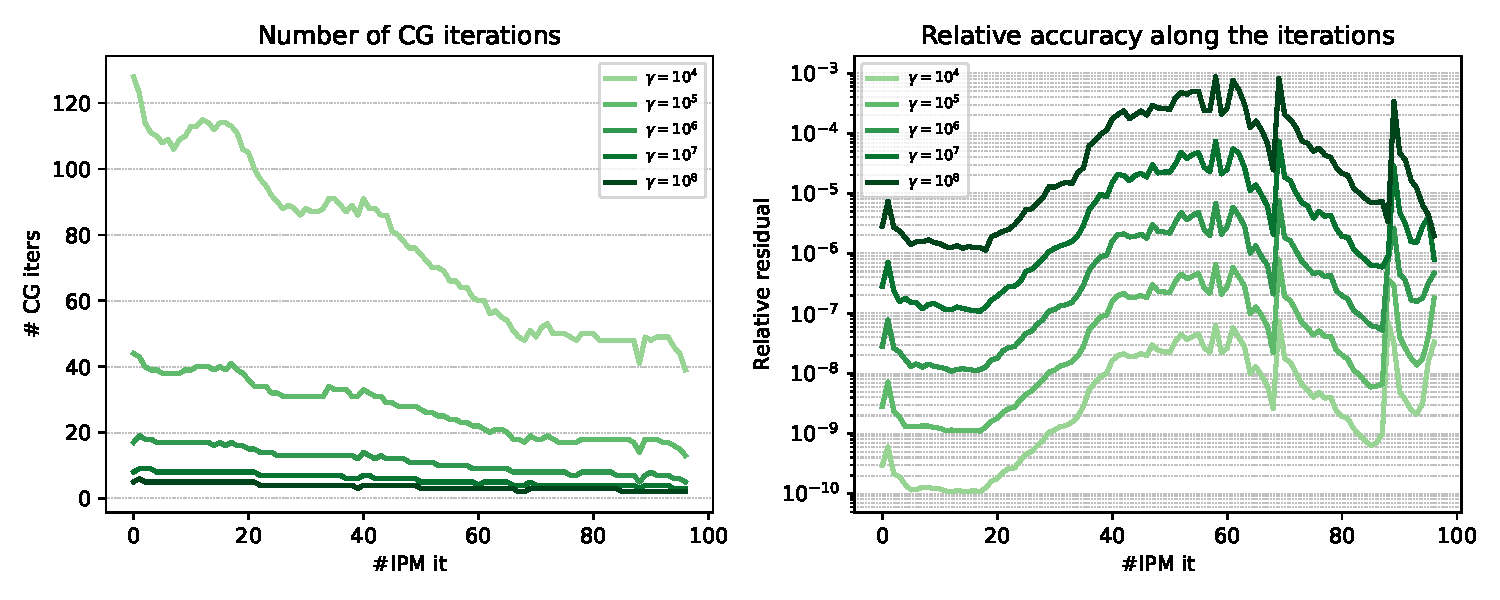
\includegraphics[width=\textwidth]{../figures/hybrid-gamma.pdf}
  \caption{
    Above: Decomposition of IPM solution time across
    (a) condensation time (cond.), (b) CG time, (c) total time
    spent in linear solver (linsol.) and (d) total time spent in
    IPM solver (IPM).
    Below: Impact of $\gamma$ on the total number of CG iterations
    and on the norm of the relative residual at each IPM iteration.
    The peak observe in the norm of the relative residual correspond
    to the primal-dual regularization performed inside the IPM algorithm,
    applied when the matrix $K_\gamma$ is not positive definite.
    \label{fig:hybrid:gamma}
    (A30 GPU)
  }
\end{figure}


\subsubsection{Tuning the equality relaxation strategy}
We now analyze the numerical performance of the equality relaxation strategy described in
Section~\ref{sec:kkt:sckkt}. The method solves the KKT system~\eqref{eq:kkt:condensed}
using a direct solver, as the relaxed problem does not have any equality constraints.
The parameter $\varepsilon$ used in the equality relaxation $-\varepsilon \leq g(x) \leq \varepsilon$
is set equal to the IPM tolerance $\varepsilon_{tol}$: in practice, it does not
make sense to set a parameter $\varepsilon$ below the IPM tolerance as the
inequality constraints are satisfied only up to a tolerance $\pm \varepsilon_{tol}$
in IPM.

We compare the performance obtained by the equality relaxation strategy
in Table~\ref{tab:sckkt:performance}, for different values of $\varepsilon_{tol}$.
We display both the runtimes on the CPU (using CHOLMOD) and on the GPU
(using cuDSS), as well as the relative accuracy achieved as we decrease the tolerance
$\varepsilon_{tol}$: we compare the solution
returned by the equality relaxation strategy together
with the solution returned by MadNLP when running on the CPU
with HSL MA27 for a tight tolerance ($\varepsilon_{tol} = 10^{-8}$).
We observe that we cannot solve the relaxed problem in MadNLP
with a tolerance below $10^{-5}$. Indeed, the slacks associated
to the relaxed equality constraints $-\varepsilon \leq g(x) \leq \varepsilon$
are converging to a value below $2 \varepsilon$ at the optimum,
leading to highly ill-conditioned terms in the diagonal matrices
$\Sigma_s$: despite being easier to solve, the conditioning
of the relaxed problem is preventing the IPM solver to converge
to a solution more accurate than $10^{-5}$.

This observation is corroborated by the results in Table~\ref{tab:sckkt:performance}.
Overall, we observe that the method is converging fast
if the tolerance $\varepsilon_{tol}$ is above $10^{-4}$.
The method benefits from the GPU-accelerated linear solver cUDSS, as
the running time decreases by a factor of 4 compared to CHOLMOD
running on the CPU. However, the method remains inaccurate:
for $\varepsilon_{tol} = 10^{-4}$, we get a $0.5$\% error on the objective,
and a $10$\% error on the primal solution.
To achieve convergence for the lower tolerance $\varepsilon_{tol} = 10^{-5}$,
we had to decrease the tolerance of the iterative refinement
to $10^{-12}$ to get a solution accurate enough in the linear solve:
this explains the significant slowdown, as we have to perform more
backsolve per iteration thanks to the additional iterative refinement
iterations.

\begin{table}[!ht]
  \centering
  \resizebox{.8\textwidth}{!}{
  \begin{tabular}{|l|rr|rr|rr|}
    \hline
    & \multicolumn{2}{c|}{\bf CPU (CHOLMOD)} & \multicolumn{2}{c|}{\bf CUDA (cuDSS)} & \multicolumn{2}{c|}{\bf accuracy} \\
    \hline
    $\varepsilon_{tol}$ & \#it & time (s) & \#it & time (s) & $\delta_{obj}$ & $\delta_{x}$ \\
    \hline
    $10^{-2}$ & 86  & 11.7 & 86  & 1.9  & $3.4 \times 10^{-1}$ & 0.66 \\
    $10^{-3}$ & 85  & 11.7 & 85  & 1.8  & $3.9 \times 10^{-2}$ & 0.22 \\
    $10^{-4}$ & 88  & 14.1 & 86  & 2.1  & $4.1 \times 10^{-3}$ & 0.10 \\
    $10^{-5}$ & 140 & 38.0 & 184 & 11.7 & $4.6 \times 10^{-4}$ & 0.06 \\
    \hline
  \end{tabular}
  }
  \label{tab:sckkt:performance}
  \caption{TO UPDATE XXX Performance of the equality-relaxation
    strategy as we decrease the IPM tolerance $\varepsilon_{tol}$.
    The table displays the wall time on the CPU (using CHOLMOD)
    and on the GPU (using cuDSS). We display the
    relative errors on the objective $\delta_{obj} = (f(x_{hsl}^\sharp) - f(x_{sc}^\sharp))/f(x_{hsl}^\sharp)$
    and on the primal solution $\delta_x = \|x_{hsl}^\sharp - x_{sc}^\sharp\|_\infty
    / \|x_{hsl}^\sharp\|_\infty$. (A30 GPU)
  }
\end{table}


\subsubsection{Breakdown of the time spent in one IPM iteration}
Now, we decompose the total wall running time spent at a single
IPM iteration, for the different linear solvers we have at our disposal.
We look at the 5th IPM iteration obtained when solving {\tt 78484epigrids}.
The results are displayed in Figure~\ref{fig:timebreakdown}. We observe
that building the KKT system represents only a fraction of the computation time, compared
to the factorization and the backsolve. The solver {\tt cuDSS} is significantly
faster to refactorize the KKT system, compared to the other linear solvers running on the CPU (MA27 and CHOLMOD).
The backsolve is the bottleneck operation for HyKKT, as it has to run a
full CG algorithm to solve the system~\eqref{eq:kkt:schurcomplhykkt}. Hence, the performance
of the HyKKT algorithm significantly improves if we manage to reduce the total
number of iterations in the CG algorithm, e.g. by increasing the parameter $\gamma$.

\begin{figure}[!ht]
  \centering
  \resizebox{.7\textwidth}{!}{
    \begin{tabular}{|l|rrrr|}
      \hline
       & build (s) & factorize (s) & backsolve (s) & accuracy \\
      \hline
      hsl        & $3.15\times 10^{-2}$&$1.22 \times 10^{-0} $&$3.58\times 10^{-1}$&$5.52\times 10^{-7}$\\
    sckkt-cpu  & $8.71\times 10^{-2}$&$6.08\times 10^{-1}$&$2.32\times 10^{-1}$&$3.73\times 10^{-9}$\\
    hckkt-cpu  & $7.97\times 10^{-2}$&$6.02\times 10^{-1}$&$7.30\times 10^{-1}$&$3.38\times 10^{-3}$\\
    sckkt-cuda & $2.09\times 10^{-3}$&$4.37\times 10^{-2}$&$3.53\times 10^{-2}$&$4.86\times 10^{-9}$\\
    hckkt-cuda & $1.86\times 10^{-3}$&$3.38\times 10^{-2}$&$1.35\times 10^{-1}$&$3.91\times 10^{-3}$\\
      \hline
    \end{tabular}
  }
  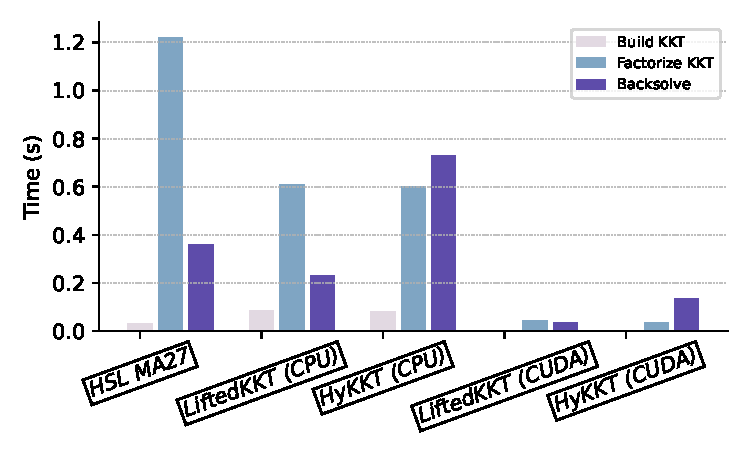
\includegraphics[width=.7\textwidth]{../figures/breakdown.pdf}
  \caption{Breakdown of the time spent in one IPM iteration
    for different linear solvers, when solving {\tt 78484epigrids} (A30 GPU)
  \label{fig:timebreakdown}}
\end{figure}



\subsection{Benchmark on OPF instances}
% The previous subsection has detailed the performance of the two KKT solvers on a specific instance, and highlighted
% the respective downsides of the Golub \& Greif strategy and the equality relaxation strategy.
Now, we run a full benchmark on difficult OPF instances taken
from the PGLIB benchmark~\cite{babaeinejadsarookolaee2019power}.
We compare our two condensed-space methods with HSL MA27 running
on the CPU. The results are displayed in Table~\ref{tab:opf:benchmark}
for an IPM tolerance set to $10^{-4}$.
We complement the table with a Dolan \& Moré performance profile~\cite{dolan2002benchmarking} displayed
in Figure~\ref{fig:opf:pprof}.

Overall, the performance of HSL MA27 is consistent with what was reported
in \cite{babaeinejadsarookolaee2019power}. We observe that HSL MA57 is slower
than HSL MA27 on this particular benchmark, as the OPF instances are super-sparse:
hence, the block elimitation algorithm implemented in HSL MA57 is not beneficial there
\footnote{Personal communication with Iain Duff.}. In addition, we observe that
the automatic differentiation is not the bottleneck in that benchmark, as it contributes to less than 10\% of
the running time on the CPU, and it parallelizes effectively on the GPU when we use ExaModels.

Overall, the equality relaxation strategy gives good results and is faster than
the Golub \& Greif strategy on small and medium instances: indeed, the algorithm
does not have to run a CG algorithm at each IPM iteration, limiting the number
of backsolves to one. However, the method solves only a relaxation of the original
problem, and suffers from the limited accuracy of the equality relaxation strategy:
the algorithm converges in 811 iterations for {\tt 30000\_goc}, leading to a slower
solution time than with HSL ma27.

Regarding HyKKT, we manage to solve all the instances for $\gamma = 10^7$, limiting
the need to tune the parameter $\gamma$ on that particular benchmark. The algorithm
is significantly faster than HSL MA27, but it remains on average slightly slower
than the equality relaxation strategy: the algorithm's weakness is the multiple
backsolves computed at each IPM iteration. For example, compared
to the other instances, the solution of {\tt 8387\_pegase} is impaired
by a larger total number of CG iterations leading to a 4x slowdown compared
to the equality relaxation strategy.
Nevertheless, the performance of HyKKT is better on the largest instances,
with almost an 8x speed-up compared to the reference HSL MA27.

\begin{table}[!ht]
  \centering
  \resizebox{\textwidth}{!}{
		\begin{tabular}{|l|rrr >{\bfseries}r|rrr >{\bfseries}r|rrr >{\bfseries}r|}
			\hline
& \multicolumn{4}{c|}{\bf HSL MA27} &
			\multicolumn{4}{c|}{\bf eq. relaxation+cuDSS} &
			\multicolumn{4}{c|}{\bf HyKKT+cuDSS} \\
			\hline
			Case & it & AD & lin & total & it & AD & lin & total & it & AD & lin & total \\
			\hline
89\_pegase & 30 & 0.00 & 0.02 & 0.03 & 28 & 0.02 & 0.03 & 0.13 & 30 & 0.03 & 0.06 & 0.17 \\
179\_goc & 43 & 0.00 & 0.03 & 0.05 & 30 & 0.02 & 0.04 & 0.14 & 43 & 0.03 & 0.06 & 0.20 \\
500\_goc & 35 & 0.01 & 0.08 & 0.12 & 36 & 0.02 & 0.04 & 0.19 & 35 & 0.03 & 0.06 & 0.20 \\
793\_goc & 31 & 0.01 & 0.10 & 0.15 & 33 & 0.02 & 0.05 & 0.20 & 31 & 0.03 & 0.08 & 0.23 \\
1354\_pegase & 42 & 0.03 & 0.29 & 0.42 & 44 & 0.04 & 0.08 & 0.32 & 42 & 0.04 & 0.14 & 0.39 \\
			\hline
2000\_goc & 38 & 0.05 & 0.57 & 0.79 & 36 & 0.03 & 0.07 & 0.31 & 38 & 0.03 & 0.13 & 0.42 \\
2312\_goc & 38 & 0.05 & 0.50 & 0.69 & 38 & 0.03 & 0.10 & 0.35 & 38 & 0.03 & 0.18 & 0.46 \\
2742\_goc & 121 & 0.27 & 3.52 & 5.22 & - & - & - & - & - & - & - & - \\
2869\_pegase & 51 & 0.10 & 0.97 & 1.34 & 52 & 0.04 & 0.14 & 0.50 & 51 & 0.05 & 0.26 & 0.65 \\
3022\_goc & 47 & 0.08 & 0.80 & 1.11 & 43 & 0.03 & 0.12 & 0.44 & 47 & 0.04 & 0.19 & 0.54 \\
			\hline
3970\_goc & 44 & 0.12 & 1.71 & 2.35 & 44 & 0.04 & 0.14 & 0.57 & 44 & 0.04 & 0.23 & 0.70 \\
4020\_goc & 57 & 0.17 & 3.62 & 4.41 & 68 & 0.06 & 0.36 & 1.00 & 57 & 0.06 & 0.41 & 1.02 \\
4601\_goc & 66 & 0.20 & 2.79 & 3.70 & 71 & 0.06 & 0.22 & 0.82 & 66 & 0.06 & 0.38 & 1.01 \\
4619\_goc & 46 & 0.16 & 2.90 & 3.67 & 54 & 0.04 & 0.20 & 0.77 & 46 & 0.05 & 0.32 & 0.89 \\
4837\_goc & 55 & 0.18 & 2.26 & 3.12 & 57 & 0.05 & 0.33 & 0.89 & 55 & 0.05 & 0.37 & 0.93 \\
			\hline
4917\_goc & 55 & 0.16 & 1.67 & 2.45 & 48 & 0.04 & 0.19 & 0.64 & 55 & 0.05 & 0.30 & 0.80 \\
5658\_epigrids & 46 & 0.18 & 2.45 & 3.35 & 50 & 0.05 & 0.28 & 0.86 & 46 & 0.05 & 0.35 & 0.94 \\
7336\_epigrids & 45 & 0.22 & 3.13 & 4.18 & 46 & 0.05 & 0.30 & 1.00 & 45 & 0.05 & 0.38 & 1.07 \\
8387\_pegase & 70 & 0.44 & 4.99 & 7.07 & 67 & 0.08 & 0.82 & 1.93 & 70 & 0.08 & 6.86 & 7.97 \\
9241\_pegase & 62 & 0.44 & 5.22 & 7.23 & 63 & 0.08 & 0.73 & 1.86 & 62 & 0.07 & 1.14 & 2.27 \\
			\hline
9591\_goc & 64 & 0.45 & 10.40 & 12.31 & 69 & 0.07 & 0.60 & 1.78 & 64 & 0.08 & 0.87 & 2.03 \\
10000\_goc & 75 & 0.44 & 5.26 & 7.31 & 56 & 0.08 & 0.30 & 1.10 & 75 & 0.09 & 0.86 & 1.88 \\
10192\_epigrids & 50 & 0.42 & 6.94 & 8.80 & 52 & 0.08 & 0.46 & 1.55 & 50 & 0.08 & 0.79 & 1.87 \\
10480\_goc & 65 & 0.54 & 10.71 & 13.15 & 71 & 0.09 & 0.93 & 2.37 & 65 & 0.08 & 1.21 & 2.57 \\
13659\_pegase & 57 & 0.55 & 6.28 & 8.77 & 65 & 0.09 & 1.70 & 3.17 & 57 & 0.07 & 1.16 & 2.64 \\
			\hline
19402\_goc & 70 & 1.20 & 31.11 & 35.93 & 108 & 0.18 & 4.95 & 8.37 & 70 & 0.12 & 2.38 & 4.84 \\
20758\_epigrids & 46 & 0.80 & 12.36 & 15.83 & 2838 & 4.63 & 325.55 & 407.69 & 46 & 0.08 & 1.83 & 3.65 \\
30000\_goc & 130 & 2.66 & 37.02 & 45.88 & 158 & 0.34 & 5.56 & 9.19 & 130 & 0.24 & 4.05 & 7.23 \\
78484\_epigrids & 96 & 7.17 & 166.35 & 192.70 & 128 & 0.48 & 15.97 & 27.49 & 96 & 0.41 & 9.75 & 19.58 \\
			\hline
		\end{tabular}
  }
  \caption{OPF benchmark \label{tab:opf:benchmark}, solved with a tolerance {\tt tol=1e-4}. (A30 GPU)}
\end{table}

\begin{figure}[!ht]
  \centering
  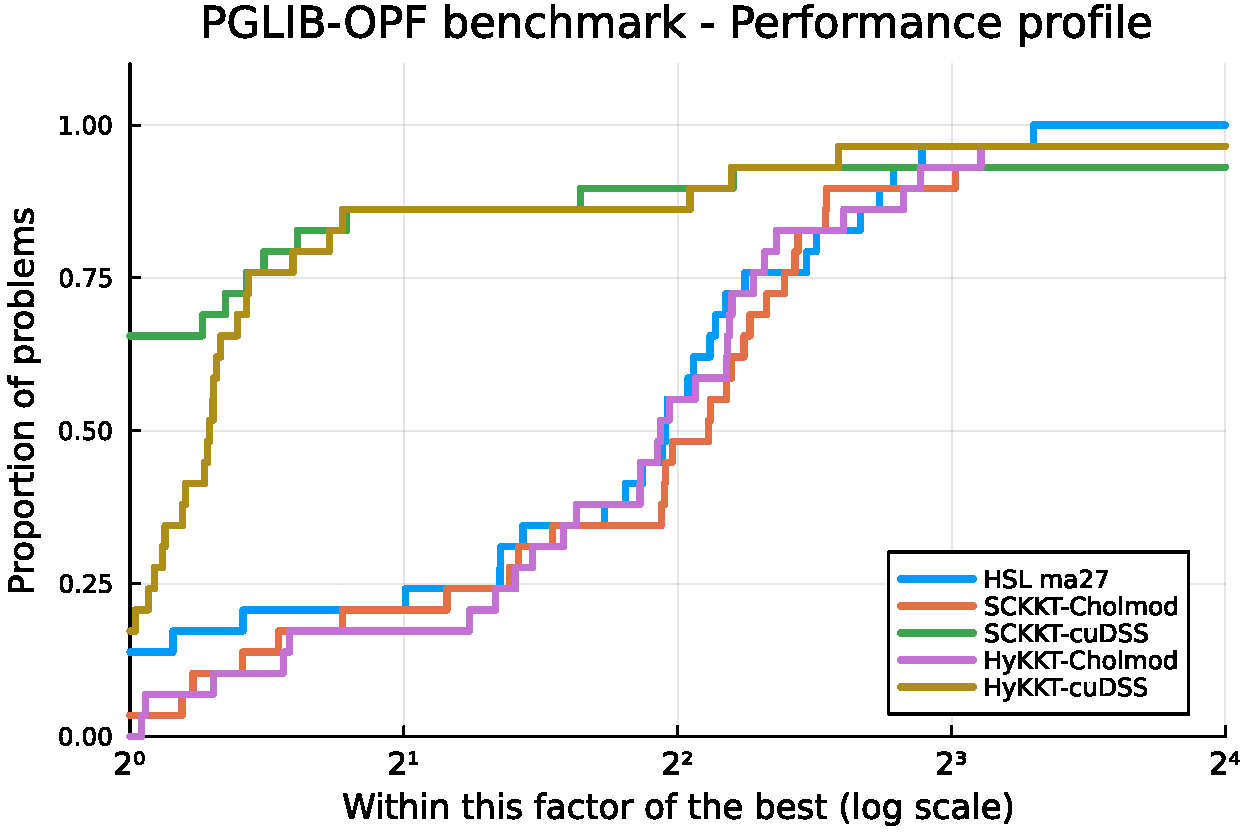
\includegraphics[width=.6\textwidth]{../figures/pprof.pdf}
  \caption{Performance profile for the PGLIB OPF benchmark, solved
    with a tolerance {\tt tol=1e-4}.
  \label{fig:opf:pprof}}
\end{figure}


\subsection{Benchmark on COPS instances}
We have observed in the previous section that both the equality relaxation
and the HyKKT algorithm gives significant speed-up for large-scale
OPF instances, compared to HSL MA27.
However, the OPF instances are specific nonlinear problems.
For that reason, we have analyzed further the performance of
the equality relaxation and the HyKKT strategies on the COPS benchmark,
which gathers generic nonlinear programs~\cite{dolan2004benchmarking}.
In this section, we look at the performance we get on the particular COPS instances used in
the Mittelmann benchmark, widely used to benchmark nonlinear optimization
solvers~\cite{mittelmann2002benchmark}.
To illustrate the heterogeneity of the COPS instances compared to the
previous OPF problems, we display in Figure~\ref{fig:cops:nnz} the sparsity pattern of the
condensed matrices $K_\gamma$ \eqref{eq:kkt:hykkt} for one OPF instance and for multiple
COPS instances. We observe that some instances ({\tt bearing}) have a sparsity pattern
similar to the OPF instance on the left, whereas some are fully dense ({\tt elec}).
On the opposite, the optimal control instances ({\tt marine}, {\tt pinene}) are
highly sparse and have highly structured Cholesky lower triangular factors.
The results of the COPS benchmark are displayed in Table~\ref{tab:cops:benchmark}.

As expected, the results are different than the previous OPF benchmark.
We observe that HyKKT+cuDSS and SCKKT+cuDSS outperform HSL MA27 on the dense instance {\tt elec}
(25x speed-up) and {\tt bearing} (6x speed-up) --- an instance whose sparsity pattern
is closed to the OPF. In the other instances, both HyKKT+cuDSS and SCKKT+cuDSS are
on par with HSL ma27 and sometimes even slightly slower ({\tt steering}).
In addition, the two solvers HyKKT+cholmod and SCKKT+cholmod offer approximatively
the same performance as HyKKT+cuDSS and SCKKT+cuDSS, respectively, indicating that these
particular instances are less amenable to GPU acceleration.

\begin{figure}[!ht]
  \centering
  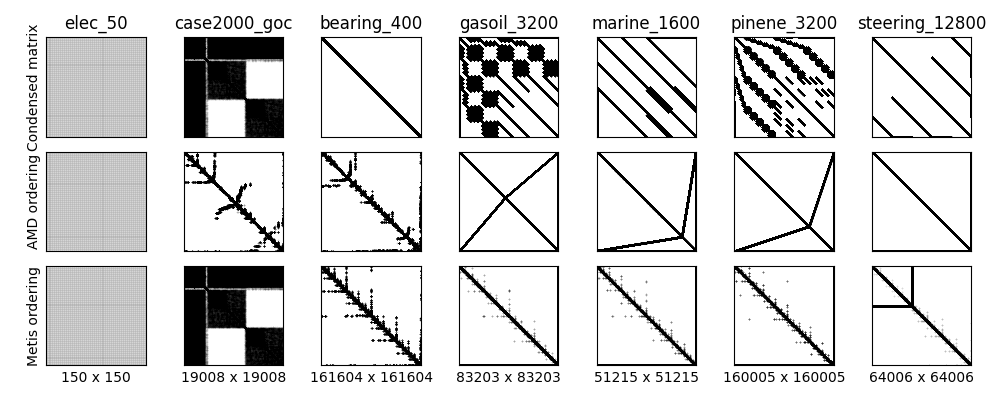
\includegraphics[width=.9\textwidth]{../figures/sparsity_pattern.png}
  \caption{Sparsity patterns for one OPF instance and for various
    COPS problems. The first row displays the sparsity pattern
    of $K_\gamma$, after AMD reordering. The second row displays
    the sparsity pattern of the triangular factor computed by CHOLMOD.
    \label{fig:cops:nnz}
  }
\end{figure}


\begin{table}[!ht]
  \centering
  \resizebox{\textwidth}{!}{
    \begin{tabular}{|l|rr >{\bfseries}r|rr >{\bfseries}r|rr >{\bfseries}r|rr >{\bfseries}r|rr >{\bfseries}r|}
    \hline
    & \multicolumn{3}{c|}{\bf HSL MA27} &
			\multicolumn{3}{c|}{\bf SCKKT+cholmod} &
			\multicolumn{3}{c|}{\bf SCKKT+cuDSS} &
			\multicolumn{3}{c|}{\bf HyKKT+cholmod} &
			\multicolumn{3}{c|}{\bf HyKKT+cuDSS} \\
    \hline
                    & it & lin & total & it & lin & total & it & lin & total & it & lin & total & it & lin & total \\
    \hline
			bearing\_400 & 10 & 6.89 & 7.26 & 11 & 1.77 & 2.16 & 11 & 0.08 & 0.83 & 10 & 2.39 & 2.72 & 10 & 0.33 & 1.10 \\
			camshape\_6400 & 21 & 0.09 & 0.14 & 17 & 0.02 & 0.07 & 15 & 0.01 & 0.09 & 21 & 0.03 & 0.10 & 18 & 0.02 & 0.12 \\
			elec\_400 & 185 & 68.46 & 77.85 & 118 & 11.02 & 14.29 & 127 & 4.12 & 6.99 & 98 & 8.91 & 11.75 & 92 & 0.43 & 3.10 \\
			gasoil\_3200 & 18 & 0.88 & 7.30 & 14 & 0.51 & 0.96 & 12 & 0.06 & 0.82 & 18 & 0.88 & 1.36 & 18 & 0.29 & 1.22 \\
			marine\_1600 & 14 & 0.61 & 0.94 & 21 & 0.44 & 0.69 & 19 & 0.09 & 0.51 & 13 & 0.32 & 0.48 & 13 & 0.12 & 0.51 \\
			pinene\_3200 & 10 & 0.95 & 8.31 & 30 & 2.25 & 3.57 & 23 & 0.16 & 1.51 & 10 & 2.71 & 3.38 & 10 & 1.28 & 2.34 \\
			robot\_1600 & 61 & 0.94 & 1.28 & - & - & - & - & - & - & 57 & 0.58 & 0.80 & 49 & 0.13 & 1.17 \\
			steering\_12800 & 17 & 0.73 & 0.98 & 15 & 0.25 & 0.63 & 13 & 0.04 & 1.09 & 12 & 0.48 & 0.75 & 11 & 0.17 & 1.36 \\
    \hline
    \end{tabular}
  }
  \caption{COPS benchmark , solved with a tolerance {\tt tol=1e-4}\label{tab:cops:benchmark} (A30 GPU)}
\end{table}


% \begin{table}
%   \centering
%   \begin{tabular}{|l|rrr|rrr|}
%     \hline
%   & \multicolumn{3}{c|}{\bf HSL MA27} & \multicolumn{3}{c|}{\bf HSL MA57} \\
%   \hline
%   & it & lin & total & it & lin & total \\
%   \hline
%     bearing\_400 & 10 & 7.53 & 7.84 & 10 & 2.17 & 2.51 \\
%     camshape\_6400 & 21 & 0.08 & 0.15 & 21 & 0.09 & 0.17 \\
%     elec\_400 & 185 & 72.77 & 80.12 & 184 & 23.47 & 30.34 \\
%     gasoil\_3200 & 18 & 0.89 & 4.85 & 80 & 8.15 & 10.01 \\
%     marine\_1600 & 14 & 0.60 & 0.84 & 13 & 0.37 & 0.47 \\
%     pinene\_3200 & 10 & 1.08 & 6.22 & 10 & 0.96 & 1.28 \\
%     robot\_1600 & 61 & 0.94 & 1.26 & 66 & 0.85 & 1.03 \\
%     steering\_12800 & 17 & 0.79 & 1.06 & 17 & 1.35 & 1.73 \\
%     \hline
%   \end{tabular}
%   \caption{Comparison between HSL MA27 and MA57}
% \end{table}

%%% Local Variables:
%%% mode: latex
%%% TeX-master: "../main"
%%% End:
